% Options for packages loaded elsewhere
\PassOptionsToPackage{unicode}{hyperref}
\PassOptionsToPackage{hyphens}{url}
%
\documentclass[
  ignorenonframetext,
]{beamer}
\usepackage{pgfpages}
\setbeamertemplate{caption}[numbered]
\setbeamertemplate{caption label separator}{: }
\setbeamercolor{caption name}{fg=normal text.fg}
\beamertemplatenavigationsymbolsempty
% Prevent slide breaks in the middle of a paragraph
\widowpenalties 1 10000
\raggedbottom
\setbeamertemplate{part page}{
  \centering
  \begin{beamercolorbox}[sep=16pt,center]{part title}
    \usebeamerfont{part title}\insertpart\par
  \end{beamercolorbox}
}
\setbeamertemplate{section page}{
  \centering
  \begin{beamercolorbox}[sep=12pt,center]{part title}
    \usebeamerfont{section title}\insertsection\par
  \end{beamercolorbox}
}
\setbeamertemplate{subsection page}{
  \centering
  \begin{beamercolorbox}[sep=8pt,center]{part title}
    \usebeamerfont{subsection title}\insertsubsection\par
  \end{beamercolorbox}
}
\AtBeginPart{
  \frame{\partpage}
}
\AtBeginSection{
  \ifbibliography
  \else
    \frame{\sectionpage}
  \fi
}
\AtBeginSubsection{
  \frame{\subsectionpage}
}
\usepackage{lmodern}
\usepackage{amssymb,amsmath}
\usepackage{ifxetex,ifluatex}
\ifnum 0\ifxetex 1\fi\ifluatex 1\fi=0 % if pdftex
  \usepackage[T1]{fontenc}
  \usepackage[utf8]{inputenc}
  \usepackage{textcomp} % provide euro and other symbols
\else % if luatex or xetex
  \usepackage{unicode-math}
  \defaultfontfeatures{Scale=MatchLowercase}
  \defaultfontfeatures[\rmfamily]{Ligatures=TeX,Scale=1}
\fi
% Use upquote if available, for straight quotes in verbatim environments
\IfFileExists{upquote.sty}{\usepackage{upquote}}{}
\IfFileExists{microtype.sty}{% use microtype if available
  \usepackage[]{microtype}
  \UseMicrotypeSet[protrusion]{basicmath} % disable protrusion for tt fonts
}{}
\makeatletter
\@ifundefined{KOMAClassName}{% if non-KOMA class
  \IfFileExists{parskip.sty}{%
    \usepackage{parskip}
  }{% else
    \setlength{\parindent}{0pt}
    \setlength{\parskip}{6pt plus 2pt minus 1pt}}
}{% if KOMA class
  \KOMAoptions{parskip=half}}
\makeatother
\usepackage{xcolor}
\IfFileExists{xurl.sty}{\usepackage{xurl}}{} % add URL line breaks if available
\IfFileExists{bookmark.sty}{\usepackage{bookmark}}{\usepackage{hyperref}}
\hypersetup{
  pdftitle={EncPos},
  pdfauthor={Fernanda Lang Schumacher},
  hidelinks,
  pdfcreator={LaTeX via pandoc}}
\urlstyle{same} % disable monospaced font for URLs
\newif\ifbibliography
\usepackage{color}
\usepackage{fancyvrb}
\newcommand{\VerbBar}{|}
\newcommand{\VERB}{\Verb[commandchars=\\\{\}]}
\DefineVerbatimEnvironment{Highlighting}{Verbatim}{commandchars=\\\{\}}
% Add ',fontsize=\small' for more characters per line
\usepackage{framed}
\definecolor{shadecolor}{RGB}{248,248,248}
\newenvironment{Shaded}{\begin{snugshade}}{\end{snugshade}}
\newcommand{\AlertTok}[1]{\textcolor[rgb]{0.94,0.16,0.16}{#1}}
\newcommand{\AnnotationTok}[1]{\textcolor[rgb]{0.56,0.35,0.01}{\textbf{\textit{#1}}}}
\newcommand{\AttributeTok}[1]{\textcolor[rgb]{0.77,0.63,0.00}{#1}}
\newcommand{\BaseNTok}[1]{\textcolor[rgb]{0.00,0.00,0.81}{#1}}
\newcommand{\BuiltInTok}[1]{#1}
\newcommand{\CharTok}[1]{\textcolor[rgb]{0.31,0.60,0.02}{#1}}
\newcommand{\CommentTok}[1]{\textcolor[rgb]{0.56,0.35,0.01}{\textit{#1}}}
\newcommand{\CommentVarTok}[1]{\textcolor[rgb]{0.56,0.35,0.01}{\textbf{\textit{#1}}}}
\newcommand{\ConstantTok}[1]{\textcolor[rgb]{0.00,0.00,0.00}{#1}}
\newcommand{\ControlFlowTok}[1]{\textcolor[rgb]{0.13,0.29,0.53}{\textbf{#1}}}
\newcommand{\DataTypeTok}[1]{\textcolor[rgb]{0.13,0.29,0.53}{#1}}
\newcommand{\DecValTok}[1]{\textcolor[rgb]{0.00,0.00,0.81}{#1}}
\newcommand{\DocumentationTok}[1]{\textcolor[rgb]{0.56,0.35,0.01}{\textbf{\textit{#1}}}}
\newcommand{\ErrorTok}[1]{\textcolor[rgb]{0.64,0.00,0.00}{\textbf{#1}}}
\newcommand{\ExtensionTok}[1]{#1}
\newcommand{\FloatTok}[1]{\textcolor[rgb]{0.00,0.00,0.81}{#1}}
\newcommand{\FunctionTok}[1]{\textcolor[rgb]{0.00,0.00,0.00}{#1}}
\newcommand{\ImportTok}[1]{#1}
\newcommand{\InformationTok}[1]{\textcolor[rgb]{0.56,0.35,0.01}{\textbf{\textit{#1}}}}
\newcommand{\KeywordTok}[1]{\textcolor[rgb]{0.13,0.29,0.53}{\textbf{#1}}}
\newcommand{\NormalTok}[1]{#1}
\newcommand{\OperatorTok}[1]{\textcolor[rgb]{0.81,0.36,0.00}{\textbf{#1}}}
\newcommand{\OtherTok}[1]{\textcolor[rgb]{0.56,0.35,0.01}{#1}}
\newcommand{\PreprocessorTok}[1]{\textcolor[rgb]{0.56,0.35,0.01}{\textit{#1}}}
\newcommand{\RegionMarkerTok}[1]{#1}
\newcommand{\SpecialCharTok}[1]{\textcolor[rgb]{0.00,0.00,0.00}{#1}}
\newcommand{\SpecialStringTok}[1]{\textcolor[rgb]{0.31,0.60,0.02}{#1}}
\newcommand{\StringTok}[1]{\textcolor[rgb]{0.31,0.60,0.02}{#1}}
\newcommand{\VariableTok}[1]{\textcolor[rgb]{0.00,0.00,0.00}{#1}}
\newcommand{\VerbatimStringTok}[1]{\textcolor[rgb]{0.31,0.60,0.02}{#1}}
\newcommand{\WarningTok}[1]{\textcolor[rgb]{0.56,0.35,0.01}{\textbf{\textit{#1}}}}
\setlength{\emergencystretch}{3em} % prevent overfull lines
\providecommand{\tightlist}{%
  \setlength{\itemsep}{0pt}\setlength{\parskip}{0pt}}
\setcounter{secnumdepth}{-\maxdimen} % remove section numbering
\usepackage{verbatim}

\title{EncPos}
\author{Fernanda Lang Schumacher}
\date{23/11/2020}

\begin{document}
\frame{\titlepage}

\begin{frame}{Motivation: sleepstudy data}
\protect\hypertarget{motivation-sleepstudy-data}{}

\begin{itemize}
\tightlist
\item
  The average reaction time per day for subjects was evaluated by
  Gregory et al.~(2003) in a sleep deprivation study.
\item
  On day 0 the subjects had their normal amount of sleep and starting
  that night they were restricted to 3 hours of sleep per night for 9
  days, and the reaction time basead on a series of tests was measured
  on each day for each subject.
\item
  The data are avaliable at the R package \emph{lme4}.
\end{itemize}

\end{frame}

\begin{frame}{Motivation: sleepstudy data}
\protect\hypertarget{motivation-sleepstudy-data-1}{}

\begin{center}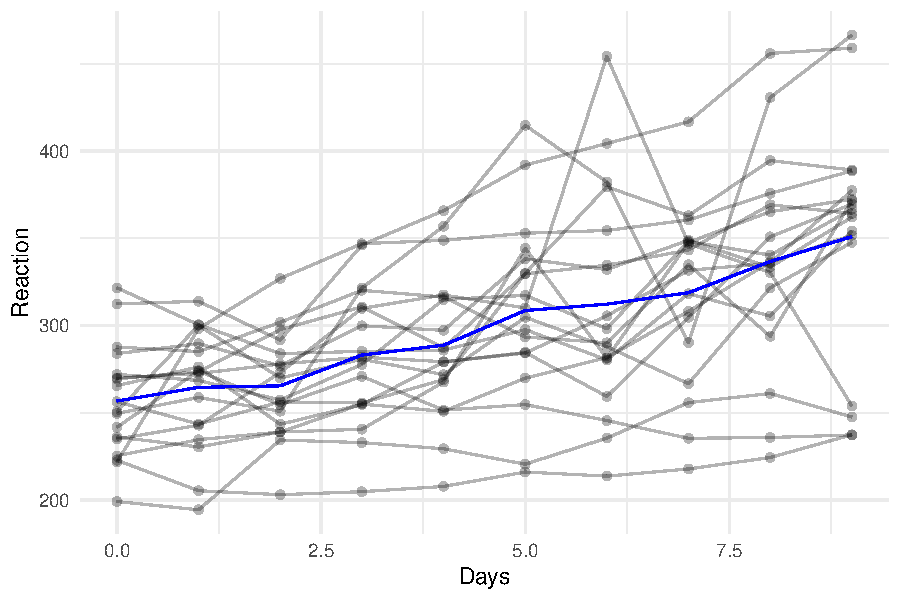
\includegraphics[width=0.85\linewidth]{codes_files/figure-beamer/data-1} \end{center}

\end{frame}

\begin{frame}{Introduction}
\protect\hypertarget{introduction}{}

\begin{itemize}
\tightlist
\item
  Bullet 1
\item
  Bullet 2
\item
  Bullet 3
\end{itemize}

\end{frame}

\begin{frame}{Linear mixed models}
\protect\hypertarget{linear-mixed-models}{}

\end{frame}

\begin{frame}[fragile]{Fitting a LMM to the sleepstudy dataset}
\protect\hypertarget{fitting-a-lmm-to-the-sleepstudy-dataset}{}

\begin{Shaded}
\begin{Highlighting}[]
\NormalTok{fit1 <-}\StringTok{ }\KeywordTok{lme}\NormalTok{(Reaction}\OperatorTok{~}\NormalTok{Days,}\DataTypeTok{data=}\NormalTok{sleepstudy,}
            \DataTypeTok{random=}\OperatorTok{~}\NormalTok{Days}\OperatorTok{|}\NormalTok{Subject)}
\end{Highlighting}
\end{Shaded}

\begin{center}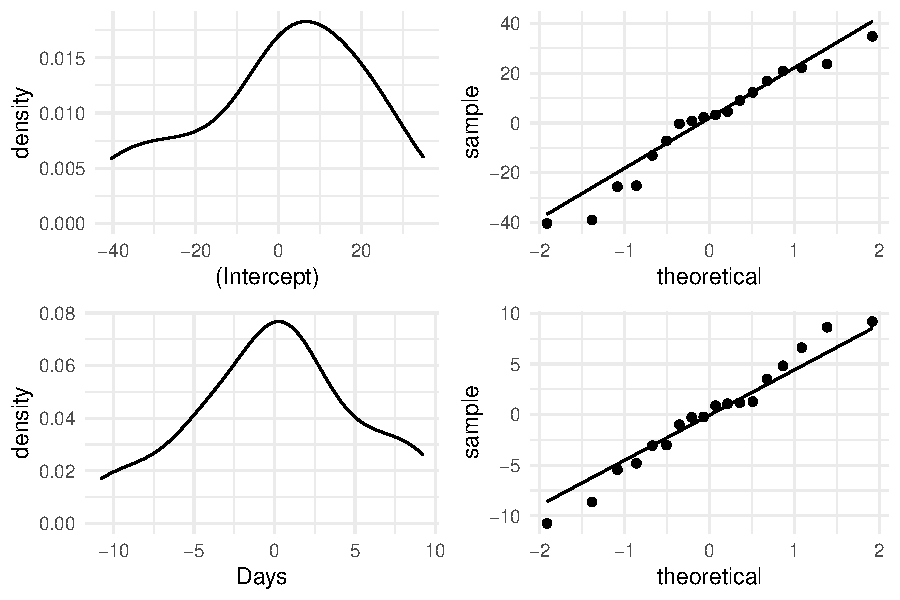
\includegraphics[width=0.7\linewidth]{codes_files/figure-beamer/fit1plot-1} \end{center}

\end{frame}

\begin{frame}{Model formulation}
\protect\hypertarget{model-formulation}{}

\end{frame}

\begin{frame}{Within-subject dependence structures}
\protect\hypertarget{within-subject-dependence-structures}{}

\end{frame}

\begin{frame}{Tools for model evaluation}
\protect\hypertarget{tools-for-model-evaluation}{}

\end{frame}

\begin{frame}[fragile]{The \texttt{R} package \emph{skewlmm}}
\protect\hypertarget{the-package}{}

\begin{itemize}
\item
  The package \emph{skewlmm} implemets an EM-type algorithm in
  \texttt{R} using S3 class, containing methods for estimating and
  predicting the SMSN-LMM.
\item
  It has an user-friendly interface with generic \texttt{R} functions
  \texttt{print}, \texttt{summary}, \texttt{plot}, \texttt{fitted},
  \texttt{residuals} and \texttt{predict} implemented.
\item
  The main functions in the package are the \texttt{smsn.lmm()} and
  \texttt{smn.lmm()} functions, which estimates the parameter of a
  SMSN-LMM and a SMN-LMM, respectively.
\end{itemize}

\end{frame}

\begin{frame}[fragile]{The \texttt{R} package \emph{skewlmm}}
\protect\hypertarget{the-package-1}{}

\begin{itemize}
\tightlist
\item
  The basic syntax of these functions is as follows:
\end{itemize}

\begin{Shaded}
\begin{Highlighting}[]
\KeywordTok{smsn.lmm}\NormalTok{(data, formFixed, groupVar, formRandom, }
\NormalTok{         depStruct, distr, ...)}
\KeywordTok{smn.lmm}\NormalTok{(data, formFixed, groupVar, formRandom, }
\NormalTok{        depStruct, distr, ...)}
\end{Highlighting}
\end{Shaded}

where

\begin{itemize}
\item
  \texttt{data}: A data frame containing all the variables to be used in
  the model.
\item
  \texttt{formFixed}: A two-sided linear formula object describing the
  fixed effects part of the model.
\item
  \texttt{groupVar}: A character containing the name of the variable
  which represents the subjects or groups in data.
\end{itemize}

\end{frame}

\begin{frame}[fragile]

\begin{itemize}
\item
  \texttt{formRandom}: A one-sided linear formula object describing the
  random effects part of the model.
\item
  \texttt{depStruct}: A character indicating which dependence structure
  should be used.
\item
  \texttt{distr}: A character indicating which distribution should be
  used.
\end{itemize}

\end{frame}

\begin{frame}{References}
\protect\hypertarget{references}{}

\begin{itemize}
\tightlist
\item
  Gregory Belenky, Nancy J. Wesensten, David R. Thorne, Maria L. Thomas,
  Helen C. Sing, Daniel P. Redmond, Michael B. Russo and Thomas J.
  Balkin (2003) Patterns of performance degradation and restoration
  during sleep restriction and subsequent recovery: a sleep
  dose-response study. Journal of Sleep Research 12, 1--12.
\end{itemize}

\end{frame}

\end{document}
